\documentclass[9pt]{beamer-control}
\usepackage{beamer-control-prac}
\begin{document}
\TOPIC[2]{Feedback Control}
\CONCEPT[3]{Week 3: Introduction to feedback}

\begin{frame}
\frametitle{Introduction}
In this practical, you will be introduced to the concept of feedback control including proportional feedback (P), integral feedback (I), and derivative feedback (D).

\vfill

This practical will consist of the following parts:
\begin{itemize}
\item Feeding back the output
\item Manual tuning
\end{itemize}
\end{frame}


\SUBCONCEPT{Feeding back the output}

\begin{frame}{Feedback}
\begin{itemize}
\item We have seen that a constant voltage input into the QUBE with the inertia disk results in an increasing angular displacement forever
\item In the case that we wish to control this angle to a particular value, this response is not very helpful and we must implement feedback control
\item We will begin by studying the effects of feeding back a proportion of the state error, the state errors derivative, and the integral of the state error
\item Once feedback has been incorporated, the input signal provides the desired output angle for the QUBE
\end{itemize}
\end{frame}

\begin{frame}{Using proportional feedback}
First let us implement a proportional feedback with gain $K_p$ to control the disk
\begin{enumerate}
	\item In Simulink, add a Gain block along with a Sum block and Slider Gain block as in the figure in the following slide. Double click on the Sum block to ensure you are using \textit{negative} feedback.
	\item You should change the step value to something other than one, double click on the Step block and change the Final value to $\tfrac{\pi}{2}$ (in Matlab/Simulink, you may use ‘pi’ for the value of pi)
\end{enumerate}
Note the proportional gain uses difference between output and the step signal to generate the “error” signal which drives the motor. The plant will then force the motor angle towards the value of the step input. The Slider Gain block is useful for adjustments during operation but is optional.
	
\textbf{Proportional control uses the \textit{present} error of the state, and acts like a spring.}
	
\end{frame}



\begin{frame}{Using proportional feedback}
	\begin{figure}
		\centering
		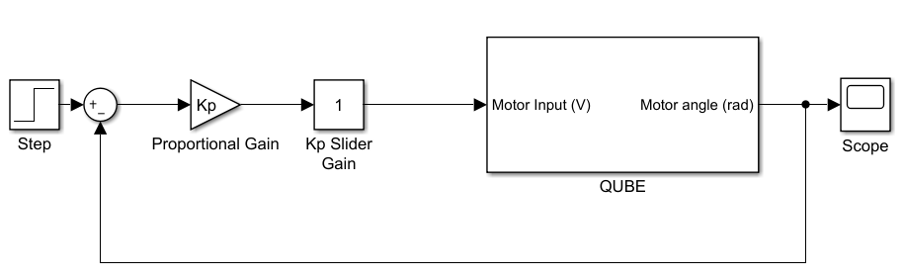
\includegraphics[width=9cm]{prac1_prop_control.png}
		\caption{Applying proportional control to the system.}
	\end{figure}
	You’ll need to select an appropriate $K_p.$ Try some large and some smaller values until you get a feel for what each of these does. You are effectively incorporating a virtual spring where $K_p$ is your stiffness. Changing the stiffness in many mechanical devices changes the way systems behave and often dictate important resonances. Hence, adding a virtual spring can be used to accomplish the same result.
\end{frame}




\begin{frame}{Using derivative feedback}
\textcolor{red}{Simulink diagram with PD control}\\
After finding a good $K_p$ we are ready to additionally implement derivative control with gain $K_d$ by feeding back the derivative of the state error (the error angular velocity in this case).

\begin{enumerate}
	\item Add a Gain block along with a Derivative block to feed back the derivative of the error signal
	\item As we are working with discretised values of angle from the angular encoder, we must first filter our signal using a low-pass filter as we saw in Week 1
	\item Find an appropriate value for $K_d$ through experimentation
\end{enumerate}

\textbf{Derivative control uses the \textit{future} error of the state, and acts like a damper opposing the velocity of the state.}
\end{frame}


\begin{frame}{Using integral feedback}
\textcolor{red}{Simulink diagram with PID control}\\
After appropriate selction of $K_d$, integral control with gain $K_i$ can be introduced by feeding back the integral of the state error. 

\begin{enumerate}
	\item The error signal can be integrated by using a Transfer Fcn block with an integrator, $G(s)=\tfrac{1}{s}$, as well as a Gain block
	\item Find an appropriate value for $K_i$ through experimentation
\end{enumerate}


\textbf{Integral control uses the \textit{past} error of the state.}
\end{frame}



\SUBCONCEPT{Manual tuning}

\begin{frame}{Hand tuning the gains}
Now that we have fully implemented PID control it is best practice to optimise the response of the plant by manually tuning the gains. 

\begin{enumerate}
	\item Adapt the PID gains to optimise performance of the controller (you may start with large variations say doubling or halving values, and then focus in with smaller variations)
	\item To assess how altering the gains affects the performance of the controller, make sure to only change one of the three gains between tests
	\item Try to achieve a step response that has minimal oscillation, has an overshoot less than 10\%, and a settling time less than 0.5 seconds
\end{enumerate}
You may wish to plot the input on the same scope as the output to better assess your controller's performance.

\end{frame}

\begin{frame}{Next week}
This week you learned how to apply P, I, and D feedback terms in a controller, and how to manually tune these gains.

Often it is very hard to tune the three gains without a good starting point. We will see in the following weeks how a model of the plant or characterisation of the output response of the plant can present initial control gains that offer acceptable control as a precursor to manual tuning. 
\end{frame}


\end{document}
